\section{EMIM-TFSI with water}
\label{section:il-h2o-structural}

ILs are, as desribed in Chapter~\ref{chapter:introduction}, one of the class of possible solvents for novel electrolytes. Despite their ionic character, also short-range interactions such as hydrogen bonds (HBs) may occur if appropriate donor and acceptor groups are present~\cite{ir-interactions-16,il-h2o-hb-il-1,il-h2o-hb-il-2,il-h2o-hb-il-3}. Due to their hydrophilic nature, ILs are usually contaminated by water, what increases the significance of HB formation for their properties~\cite{il-h2o-water-1,il-h2o-water-2,il-h2o-water-3,il-h2o-water-4,il-h2o-water-5}. One of popular ILs is EMIM-TFSI, which in pure state, was studied by MD~\cite{il-h2o-previous-work}. In this section structural results obtained form EMIM-TFSI IL with differing amount of water contamination are presented. This study was described in the article~\cite{il-h2o}.

\subsection{System details}

Studied systems contained 15 pairs of EMIM-TFSI ionic pairs and an increasing number of water molecules: 0, 2, 5 and 15, corresponding to water mole fraction $x$ equal to 0, 0.12, 0.25 and 0.5, respectively. Also, a~system of neat water containing 181 molecules was modeled. In order to average results, two independent replicas for neat liquids and three for IL/water mixtuers were simulated.

Initially, classical MD simulations were performed for equilibration for 100~ns in the NpT ensemble with pressure of 1~atm and temperature 298~K and then for 100~ns in the NVT ensemble. Next, structures from these simulations were used as starting points for AIMD in NVT ensemble with temperature of 298~K. 40~ps of trajectories were recorded, analysis was done for the last 30~ps. For both classical MD and AIMD a~timestep of~1~fs was used.

\begin{figure}[ht]
    \centering
    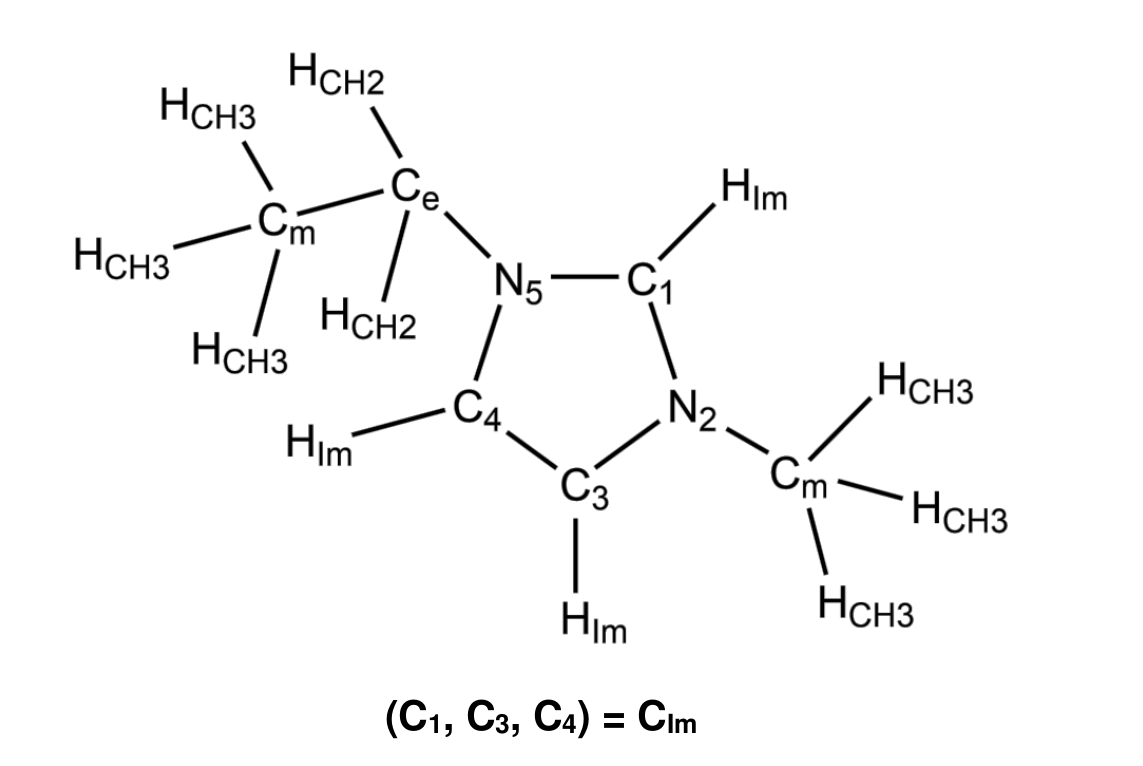
\includegraphics[width=0.4\textwidth]{img/3-structural-data-from-md-simulations/6-il-h2o/emim-labeling.png}
    \caption{Labeling of atoms in EMIM$^{+}$ cation}
    \label{fig:il-h2o-emim-labeling}
\end{figure}

Here, plots of the distribution functions were made with the use of TRAVIS~\cite{travis-1,travis-2}. In the description of results O$_{\text{TFSI}}$ means oxygen atoms from the TFSI$^{-}$ anion and O$_{\text{w}}$ oxygen atoms from water molecules. Labeling of atoms from EMIM$^{+}$ cation is presented in Figure~\ref{fig:il-h2o-emim-labeling}.

\subsection{Results}

As a~starting point for hydrogen bonding analysis, radial distribution functions are examined, plots for selected atom pairs in the system with 0.5 mole fraction of water are presented in Figure~\ref{fig:il-h2o-rdf-0.5} and for neat IL in Figure~\ref{fig:il-h2o-rdf-0.0}. For pairs involving imidazolium ring hydrogen atoms (H$_{\text{Im}}$-O$_{\text{TFSI}}$ or H$_{\text{Im}}$-O$_{\text{w}}$) the first sharp maximum appears slightly above 2~{\AA} with smaller next maxima above 4~{\AA}. For pairs with methyl hydrogen atoms (noted as H$_{\text{CH}_3}$) maxima near 2~{\AA} are weaker and the main maxima are loacted at about 4~{\AA} but still are lower than the first peak for H$_{\text{Im}}$ atoms. At H-F RDFs the behavoiur of both types of hydrogen atoms is similar with weak maxima at 3~{\AA} and main maximum between 4.5 and 5.5~{\AA}. Thus, from these functions it may be concluded, that EMIM$^{+}$ will interact with oxygen atoms from anions or water molecules, mostly by the hydrogen atoms from the imidazolium ring.

\begin{figure}
    \centering
    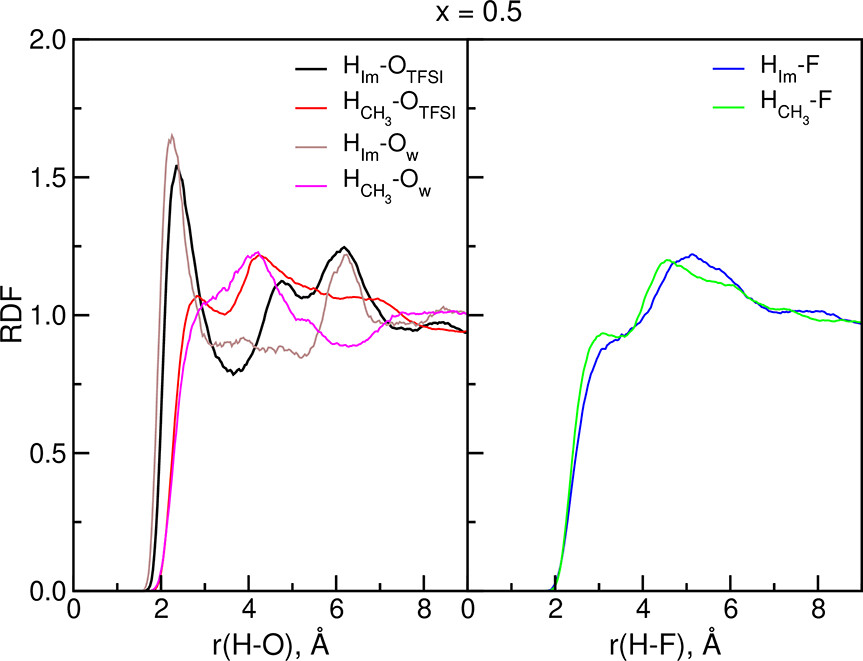
\includegraphics[width=0.6\textwidth]{img/3-structural-data-from-md-simulations/6-il-h2o/rdf-0.5.png}
    \caption{Radial distribution functions for selected atom pairs for systems with water mole fraction 0.5}
    \label{fig:il-h2o-rdf-0.5}
\end{figure}

\begin{figure}
    \centering
    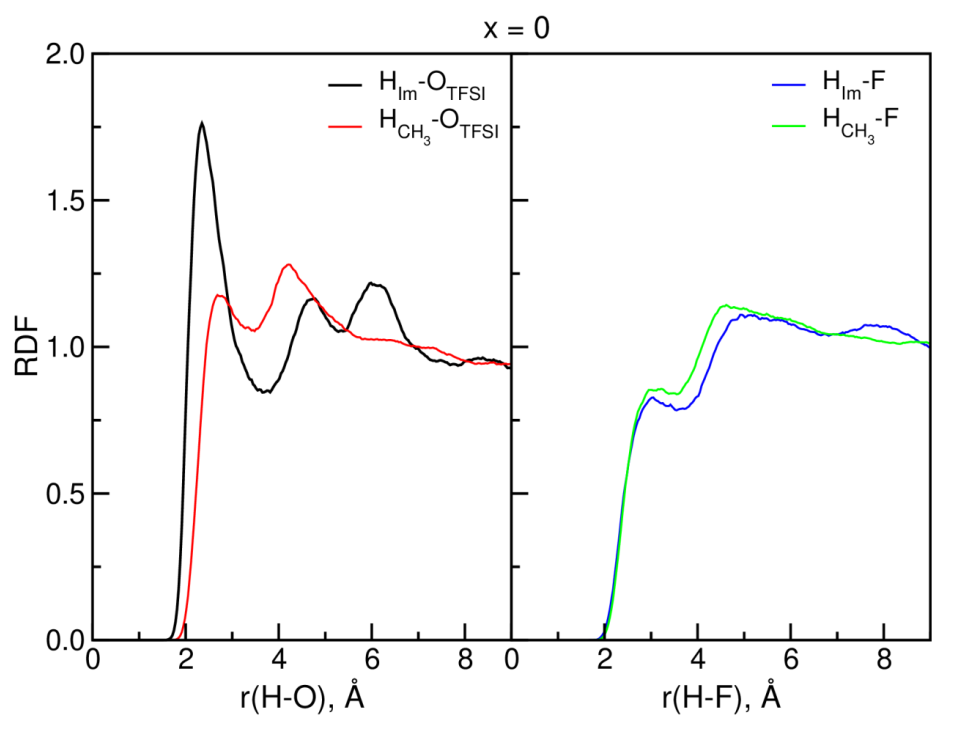
\includegraphics[width=0.6\textwidth]{img/3-structural-data-from-md-simulations/6-il-h2o/rdf-0.0.png}
    \caption{Radial distribution functions for selected atom pairs for neat IL}
    \label{fig:il-h2o-rdf-0.0}
\end{figure}

To form a~hydrogen bond (HB) it is also needed that the donor (D), acceptor (A) and hydrogen (H) atoms are in a~sufficiently linear arrangement. Therefore, for further analysis, combined distribution functions (CDFs) were plotted. They show the relative probability of finding a~configuration of atoms at a~specified D-A distance and D-H-A angle. A~sample plot for the system with $x = 0.5$ is presented in Figure~\ref{fig:il-h2o-cdf}. The preferrable values for HB are D-A distance up to 350~pm and D-H-A close to 180{\degree}. There is a~large probability of finding such configuration for C$_{\text{Im}}$-H-O$_{\text{TFSI}}$ as well as for the C$_{\text{Im}}$-H-O$_{\text{w}}$. The probability of finding appropriate configurations for C${_{\text{m}}}$ atoms is smaller but non-negligible. Occurences of C-H-F arrengements suitable for hydrogen bonding are infrequent.

\begin{figure}[ht]
    \centering
    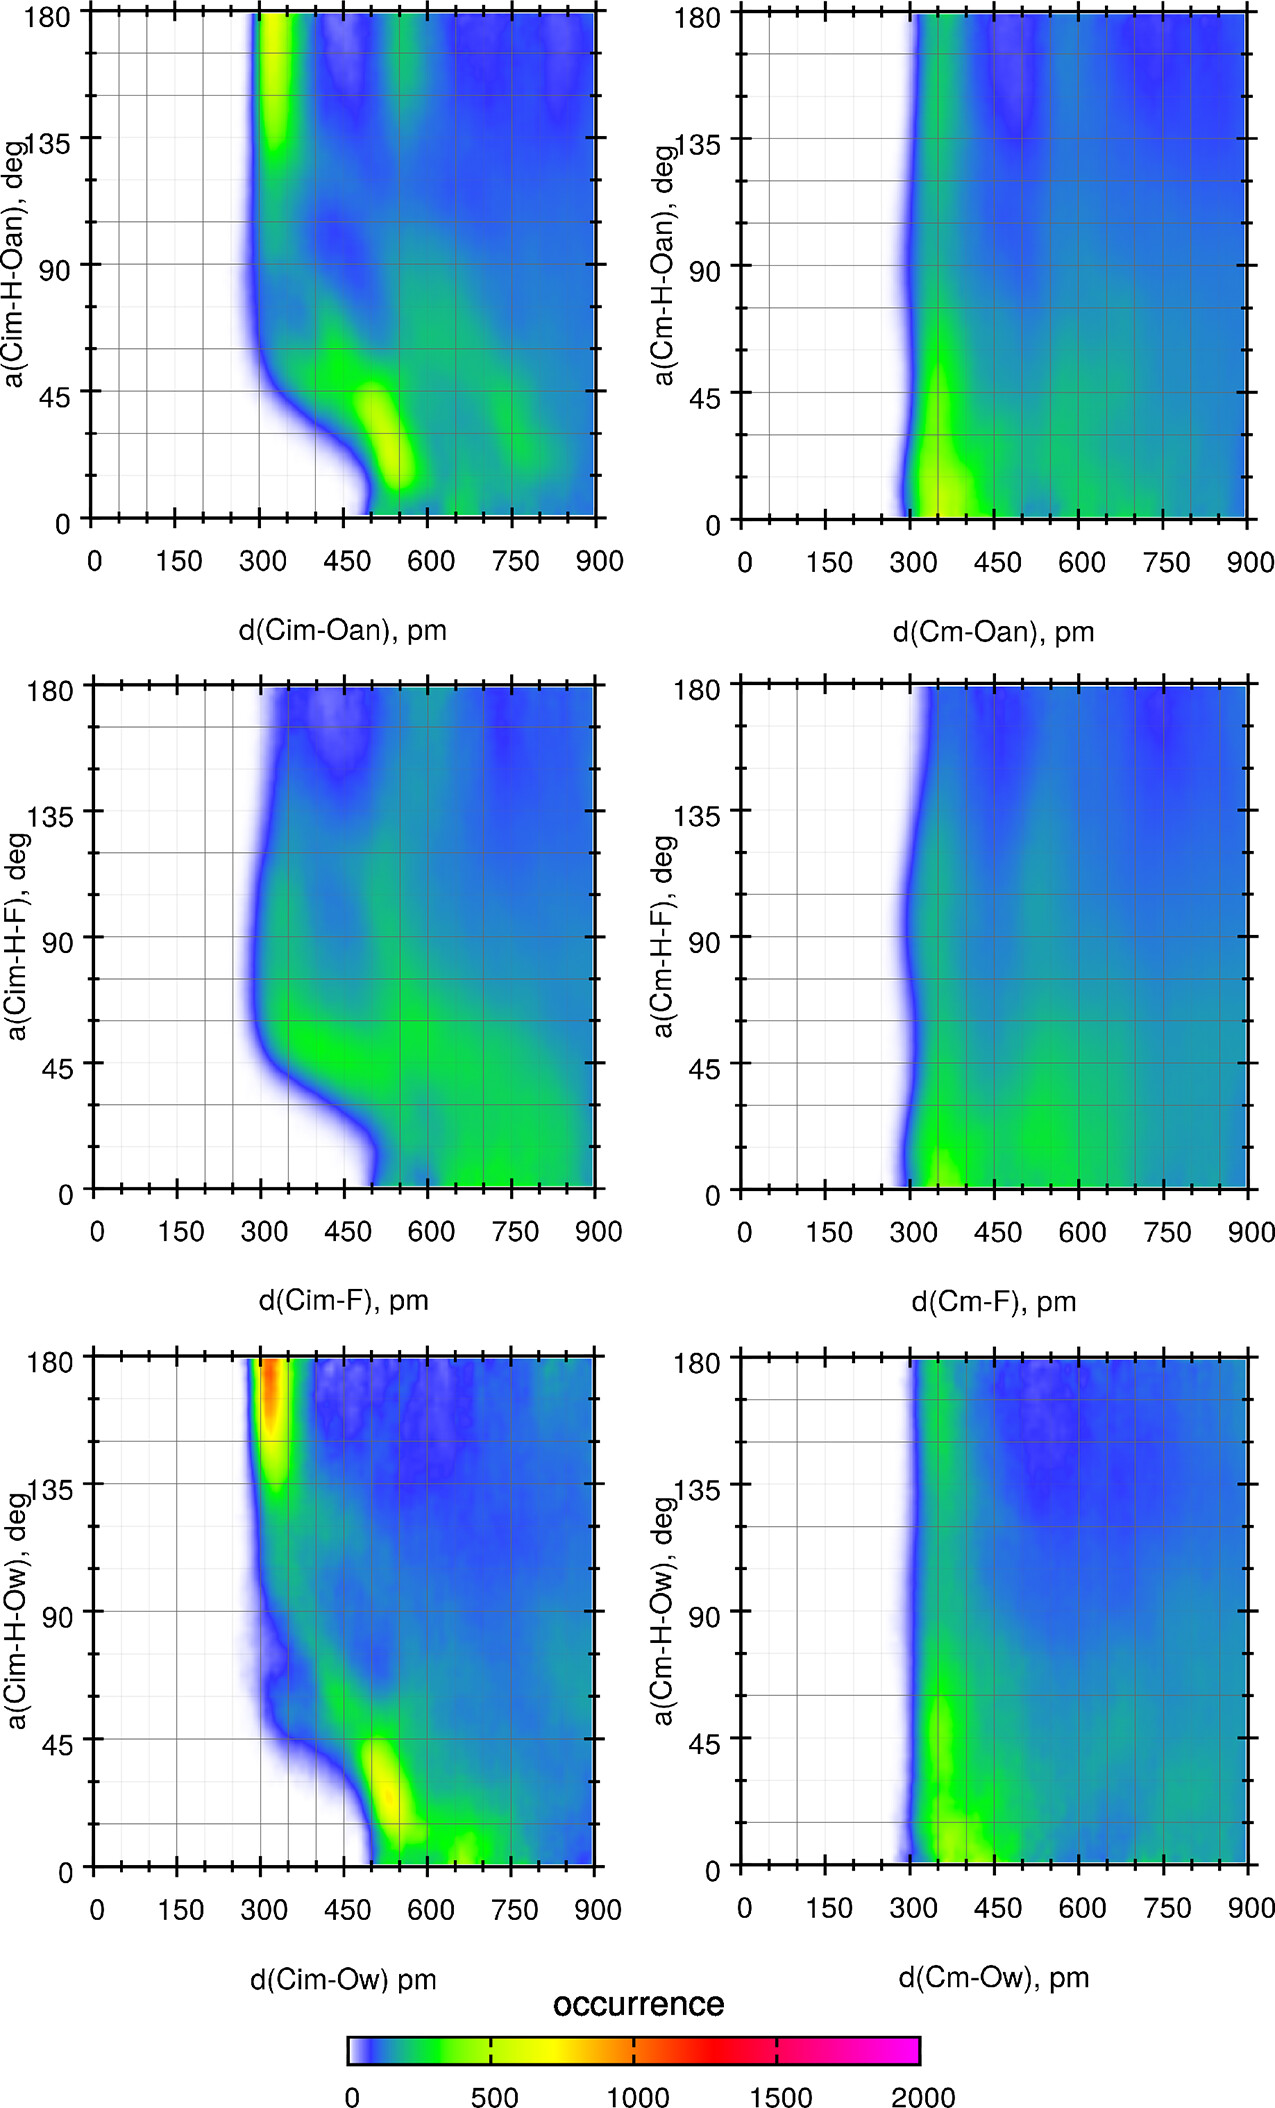
\includegraphics[width=0.50\textwidth]{img/3-structural-data-from-md-simulations/6-il-h2o/cdf-0.5.png}
    \caption{Combined distribution functions for selected donor-hydrogen-acceptor atoms in systems with water mole fraction 0.5}
    \label{fig:il-h2o-cdf}
\end{figure}

Spatial distribution functions (SDFs) plotted in Figure~\ref{fig:il-h2o-sdf} confirm previous observations - the regions of increased density of oxygen acceptors are close to hydrogen atoms from the imidazolium ring.

\begin{figure}
    \centering
    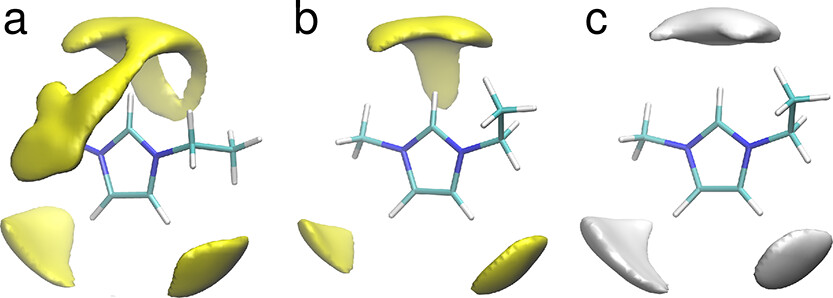
\includegraphics[width=0.5\textwidth]{img/3-structural-data-from-md-simulations/6-il-h2o/sdf.png}
    \caption{Spatial distribution functions of oxygen atoms around EMIM$^{+}$ cations: TFSI$^{-}$ anions in the neat IL (a); TFSI$^{-}$ anions in the $x = 0.5$ mixture (b); water molecules in the $x = 0.5$ mixture (c). Surfaces of particle isodensity of 10~atoms/nm$^{3}$ are shown}
    \label{fig:il-h2o-sdf}
\end{figure}

Figure~\ref{fig:il-h2o-hb-statistics} shows statistics of HBs for each system. The criteria of the existence of the HB were the following: D-A distance not larger than 3.5~{\AA} and the deviation of D-H-A angle from linearity not bigger than 40{\degree}. In the neat IL, EMIM$^{+}$ cations form 2.5~HBs per cation, 1.7 of these bonds are to oxygen atoms. About half of H-O$_{\text{TFSI}}$ bonds are formed by hydrogen atoms from the imidazolium ring. For methyl groups the average number of bonds is~0.6, here the lower probability of bonding is compensated by the bigger number of available hydrogen atoms of this type. Bonds to fluorine atoms are less probable (about 0.6 bonds per cation) and to nitrogen atoms are the least probable (0.15~per cation).

\begin{figure}
    \centering
    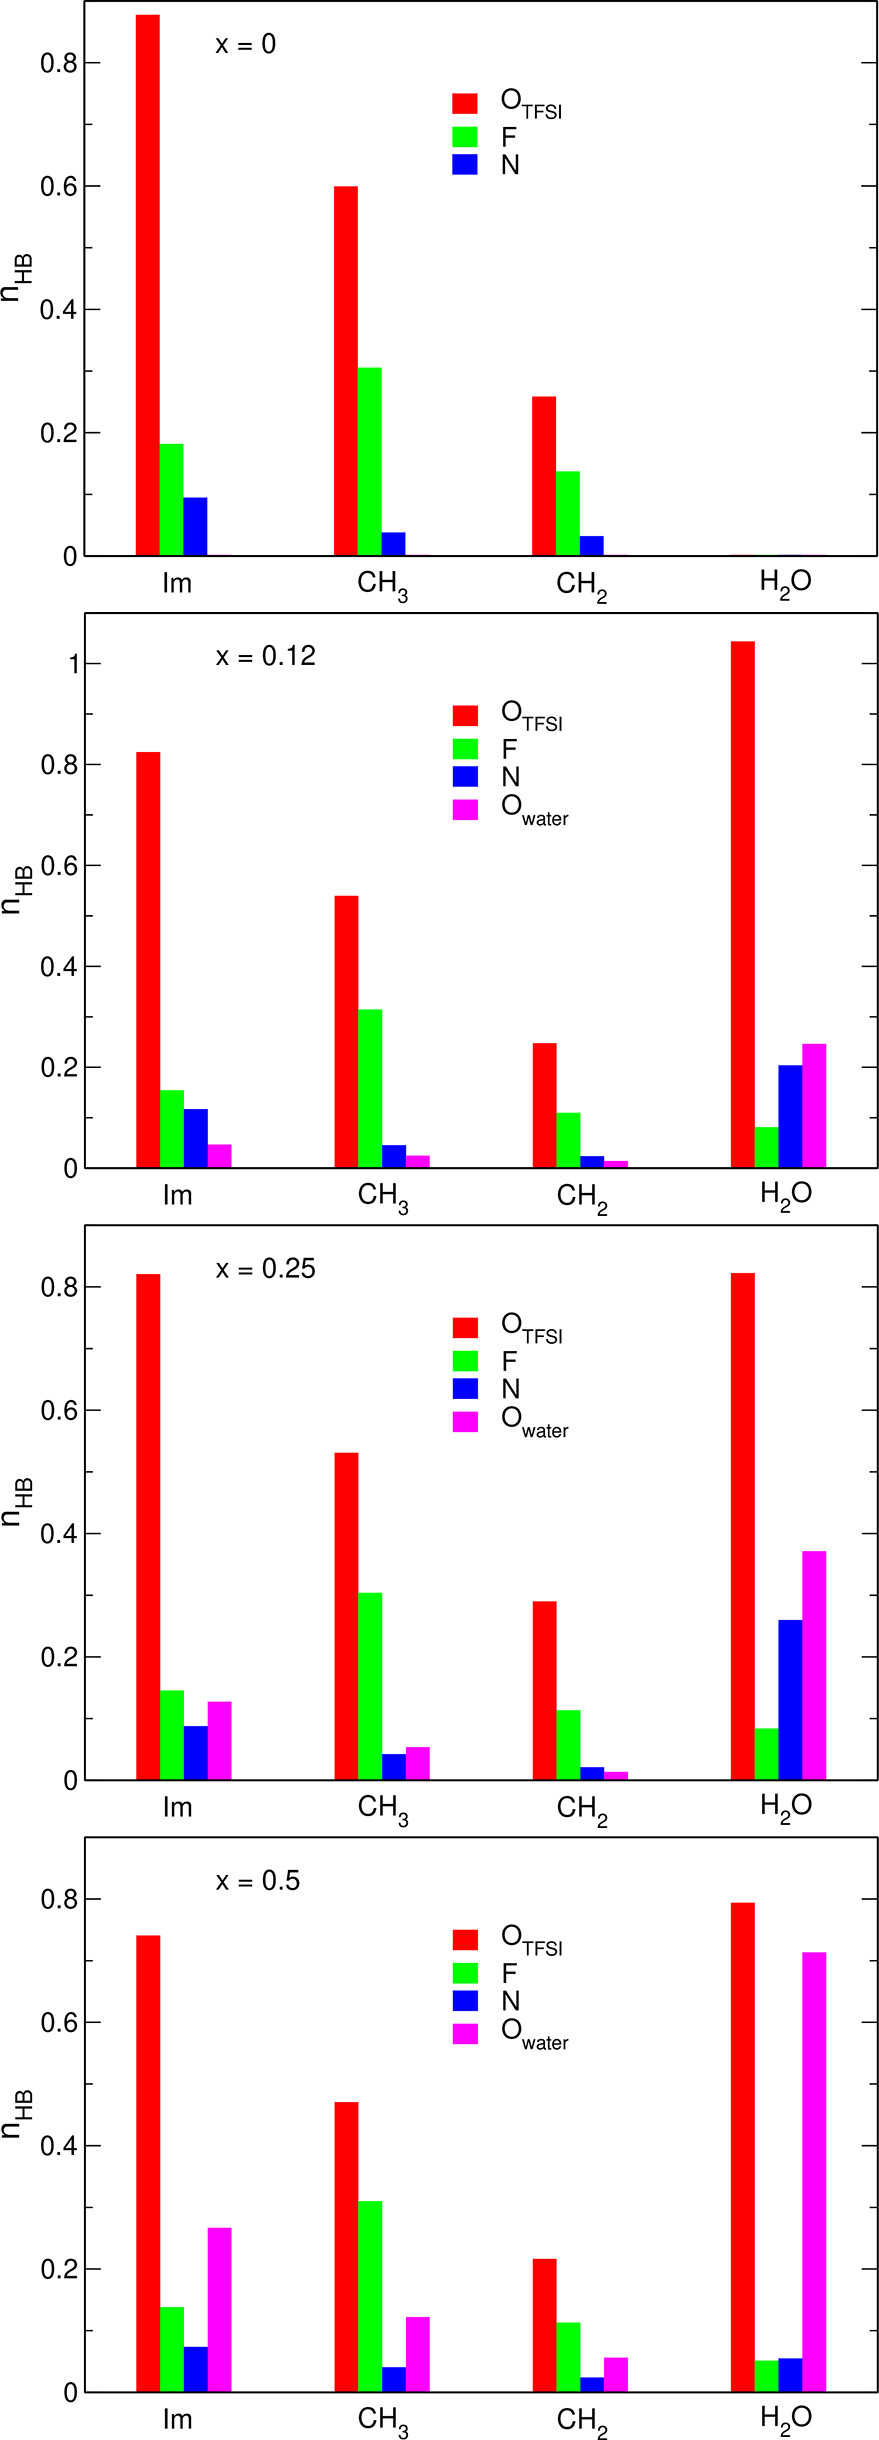
\includegraphics[width=0.5\textwidth]{img/3-structural-data-from-md-simulations/6-il-h2o/hb-statistics.png}
    \caption{Average number of hydrogen bonds $n_{\text{HB}}$ per donor. Donors are shown in the horizontal axis, acceptors are marked by colors}
    \label{fig:il-h2o-hb-statistics}
\end{figure}

In systems with water, H$_2$O molecules tend to form HBs with oxygen atoms from TFSI$^{-}$ anions, and there is about 0.8~of HB per H$_2$O molecule in system with $x = 0.25$ or $x = 0.5$. The system with $x = 0.12$ is an outlier, probably because of the poor statistics when the simulation box contains only two water molecules. For EMIM$^{+}$ cations the total number of formed HBs remains approximately unaffected and is in the range of 2.45-2.56 bond/cation. However, with increase of the content of water, there appears competition between TFSI$^{-}$ anions and water molecules and it leads to decrease of EMIM-TFSI HBs number.

With increasing concentration of water, also the probability of water-water HB increases, in the most concentrated mixture there are 0.7 such bonds per water molecule. For systems with $x = 0.12$ or $x = 0.25$ there is a~significant number of water-N bonds, about 0.25 per H$_2$O molecule and it disappears at bigger concentration. The average number of total HBs formed by water molecule is smaller in IL: 1.61 in the $x = 0.5$ system while in neat water it is equal 1.91. The number of accepting hydrogen atoms is also smaller in IL and for the most concentrated mixture is equal 1.15. 

For TFSI$^{-}$ anions the loss of EMIM-TFSI HBs is compensated by formation of water-TFSI HBs, and the average number of HBs per anion increases from 2.5 in the neat IL to 3.0 in the $x = 0.5$ system.

To summarize, in a~mixture of liquids, water molecules form less HBs than in the neat water. For EMIM$^{+}$ cation total number of HBs remains fairly constant, with some replacement of EMIM-TFSI HBs by EMIM-water HBs. In neat IL not all of the oxygen atoms in TFSI$^{-}$ anion are used for HBs, thus it gives probability for formation of additional HBs with water and the total number of HBs per anion increases with growing concentration of water. In section~\ref{section:il-h2o-ir} influence of changes in number of HBs on the IR spectrum of the system will be described.